\lhead{\emph{System Design}}
\chapter{System Design}

\section{System Components}
In this chapter we will provide an overview \autoref{fig:systemComponents} of the components of the system and their function. The overall system is divided into three components remote data collection, data transport and, the server processing and storage.  It is presumed that the remotes have varying locations (although they may stay in a single place for months or years). Remotes are not specifically tied to any geography.  They may be it marine or land based. In this discussion, examples are assumed to be a marine application.  

\begin{figure}
\centering
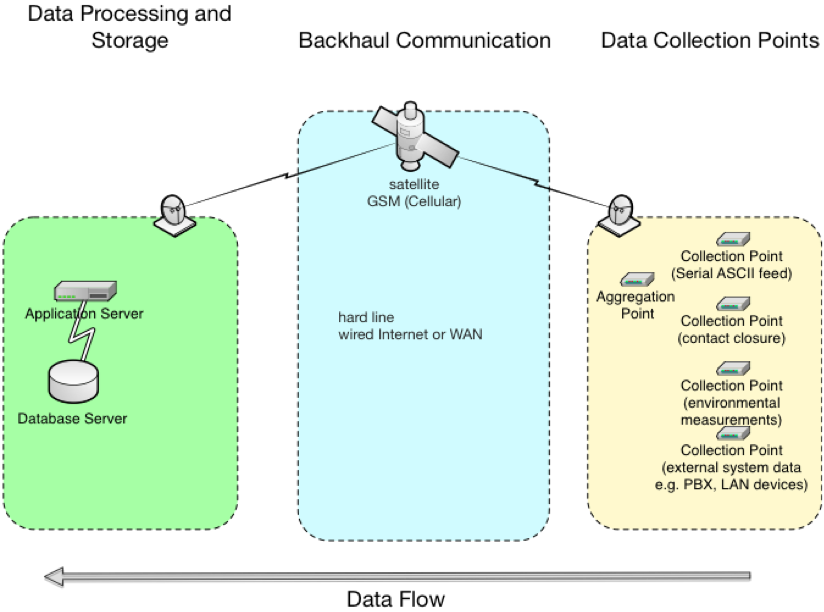
\includegraphics{Figures/systemComponentOverview}
\caption{System Components}
\label{fig:systemComponents}
\end{figure}
\section{Data Collection Component}

The layout of the data collection component tiered and resides fully on the remote site.  The devices that act as collection points are known in our system as nodes.  They are installed on-board with the tasks to receive, secure and transmit the data.  A remote site must house at least one node but may have multiple nodes installed.  Each node, in turn, is comprised of one or more data inputs called tendrils.  A tendril is a single source of data which reports directly to the node. 

\subsection{Nodes}

The node uses a small on-board device which is capable of running a general use operating system. For our mock up node, a BeagleBoard\cite{Anonymous:zgMDnVpL} brand embedded device is used.  The node is designed to have a small resource footprint with CPU, memory and storage capacity restricted and cost effective.  The device is configured with 512M of RAM, a single code CPU, and 1 Gig of SSD disk storage.  The CPU draws very little power and produces minimal heat.  This relieves a requirement for a fan in most applications and results in a device with no moving parts.  

A node may receive inputs from a variety of sources.  Each node's id is unique throughout the system.  With a unique id it is possible to have many nodes installed on a single remote site and across sites and nodes can be migrated to other sites. This proves useful in the case that a datasource is moved. For instance if a cargo container is transported to another ship. 
In our reference implementation we will limit to a single node with multiple simulated inputs.  These inputs are referred to as tendrils that are tasked to provide the events to the node.  The node will accept to a variety of different tendrils and collect their event information.  

\begin{figure}
    \centering
    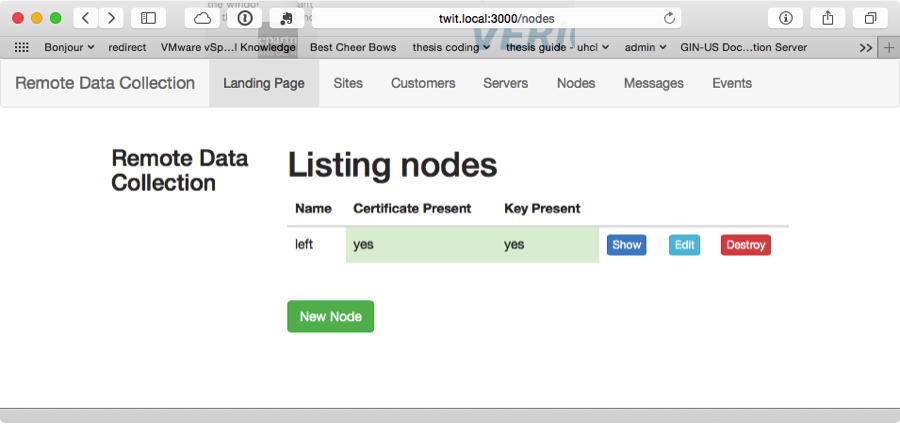
\includegraphics[scale=.9, angle=0]{Figures/interfaceNodes}
    \caption[Nodes Interface]{Web Based Interface for Node Management}
    \label{fig:interfaceNodes}
\end{figure}

\subsection{Tendrils}
The idea of the tendril is one of flexibility. 
It is designed with an abstraction layer based on the REST protocol. A wide variety of information is made possible by this design. 
Example types include Environmental, State Change Detection, Location, and events sent by intelligent systems.  
More specific examples include: ambient temperature, humidity, door openings and closures of a cargo container, GPS position, wave height, wind speed and sophisticated system activities such as phone calls and email activity. We create three types of tendril inputs although any number may be possible. Contact closure, serially attached streams, and intelligent system messages present an overview of what is possible. 
\subsubsection{Contact Closure}
Contact closures\cite{OmegaEngineeringInc:vi} in this context would have a circuit connected to a relay on a door, for example. Opening the door also creates an open circuit is detected by our agent. The event is recorded and secured on the agent with a timestamp and position if available. The purpose of such a measurement is to detect a container being accessed. The event, once processed, is compared against a policy of access that determines if the access was authorized. The converse of this is to detect events that are scheduled to occur. For example detection of a fuel cap being removed on a generator to indicate it was inspected. \autoref{fig:contactClosure} Contact closure relays are low cost devices that can be configured as a tendril\cite{Anonymous:wa}.
\begin{figure}
\centering
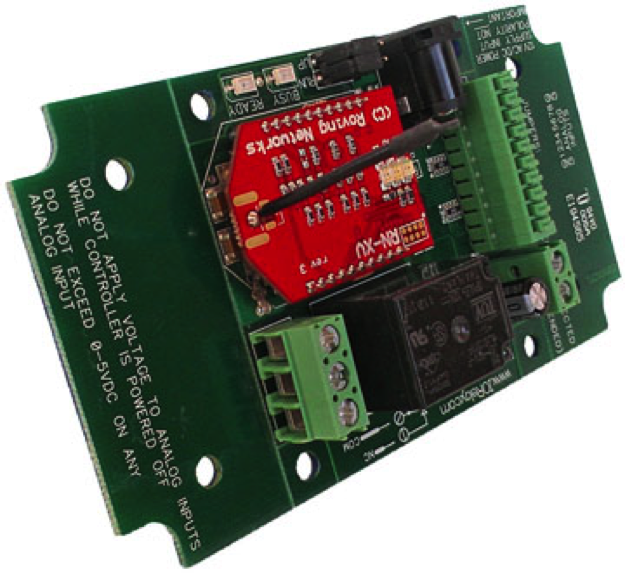
\includegraphics{Figures/contactClosure}
%\caption{Contact Closure - RelayPros R110PL_WIFI WiFi Relay}
\caption{Contact Closure - RelayPros Wifi Relay}
\label{fig:contactClosure}
\end{figure}
\subsubsection{Serially Attached Systems} 
Serially attached systems are considered to be systems attached via an RS–232 or similar pinned connection. They are devices that have a serial console connect which provides either a stream of character data or an updated status screen. An example is a GPS device which provides a NEMA string. A device in this configuration has a consistent stream of ASCII data using a standard protocol. GPS positioning coordinates as well alarms and electronic fence data are sent down the serial link to the attached node. Within the node, as with all devices, the stream data is secured in messages for transmission to the storage systems.
\subsubsection{Intelligent Systems}
We recognize a third category of tendril data sources termed intelligent systems. They have the ability to process, compile and digest their information before collection. They have significant processing power and can transmit over a local network to the local node.  
Examples of these are VoIP call managers, routing, switching, and WiFi infrastructure, and servers.  These can record call detail records for from call managers, routers and infrastructure log data, and diver / ROV  \cite{Christ:2011vn} video systems.
Potential use cases include but are certainly not limited to: Logging Environmental Systems Call Manager Systems, Email, and Cell phone usage
The end result of all this information collection with the remote is the standard interface that feeds the message. Upon. The remote upon receiving an input it will take me information contained and security and the message Block. These message locks are then either transferred immediately or stored and transferred once the system is online.
During the Deepwater Horizon explosion, many elements of data were generated leading up to the explosion itself. 
Much of this data was from the phone system and cellular network. Both of these could have been captured and transmitted up to the point that connectivity was lost. 


\section{Transmission}
The transmission component of the system, also referred to as the backhaul, can be provided by a number of network topologies and technologies. Therefore we can make few assumptions about it’s quality, bandwidth, or availability. The system therefore treats the transmission component as a generic pipe. The one assumption that we do make is that the connection must be available before the node resources are exhausted. This will vary depending on the application but generically we expect communication to be resumed available every 24 to 48 hours. Practical expectation is that connectivity would be more frequent and stable.

This backhaul link is also assumed to be inherently insecure. Public networks such as the Internet and cellular phone networks will be routinely used. Therefore all security is managed within the message block itself. Key exchange (key agreement) is provided using a pre-shared, symmetric key. In this model the message processing does not require the transmission link to be online when messages session key is created.

\section{Storage and Processing}
The storage and processing component of the system is the server that lives within the data center. The site would be a corporate installation owned and controlled by the end user. Security of the physical system and access to the operating system are assumed.  Messages received by the server are decrypted and placed into the database. Depending on the sensitivity of the message appropriate database level encryption can be used for increased protection and prevents access by an authorized user should the system be breached. 

The storage and processing component of the system is composed of three functional pieces. At its base provides a data store for the messages to be decrypted and stored. and available for processing. Secondly, it provides the business logic interface for configured rules and their thresholds. Finally it is the user interface for provisioning and management, and key management the node devices. 

\section{Reporting}
As part of the storage and processing we expect to produce a geographic mapping application \autoref{fig:interfaceMap} to show the position of the nodes as they traverse the. 
Popup values such as online / off-line, number of messages received, and time since last contact. The interface should also provide the ability for the user to correlate events. E.g. correlate by time, by a fleet, by system type. 

\begin{figure}
\centering
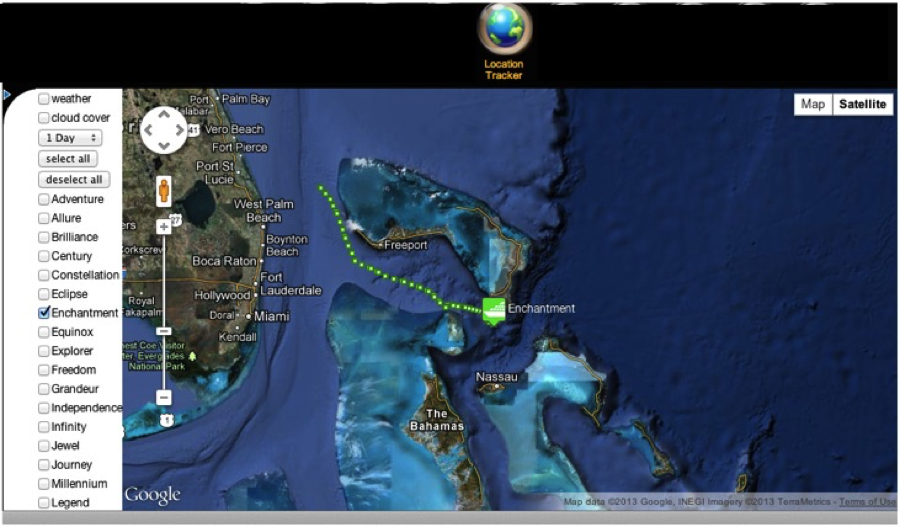
\includegraphics[scale=.9]{Figures/interfaceMap}
\caption{Map Interface}
\label{fig:interfaceMap}
\end{figure}

\section{Messages}
Requirements for our solution are securing the information at the time of collection, transmitting the information securely and, storing the information in the data center securely. To address these we have designed message formats and protocols to mitigate the threats. Our solution provides the following security attributes:  confidentiality, integrity, and non-repudiation (authentication). 

The message format is composed of the payload, and a hash message authentication code (HMAC). For the event data we look inside the payload. It contains the timestamp, ids for both the tendril and the node, and the event data itself. The event carries two fields within it didn’t type and it’s content.  To manage the data on the remote we designed process that begins with an input at the tendril. The element manager through either polling or an event will signal the node to create a message. The node then takes this event data and formats it into a message. The message format contains a hash of the payload (HMAC), which provides data integrity. (detailed below) Encryption with a shared key provides the confidentiality. Our process of key management, which is discussed below, handles origin integrity, nonrepudiation or authentication.   Once even has been processed into a message and secure, it is handed off to the transition component where it will either be transmitted immediately or store on the remote node.

\subsection{Digital Signature Algorithm}
The format supports the integrity property by default. As mentioned above, Integrity is maintained by use of a message authentication code (MAC) on the payload data. A hashed MAC (HMAC) employing SHA-2 is chosen in order to avoid known hash collision exploits found in other hashing algorithms. \cite{Turner:MiRyW-r_} 

\subsection{Encryption Algorithm}
Encryption is centered on the public/private key pair created and stored at install time of the node. A 1024k bit RSA algorithm is used to generate both a server and a node key pair. 

The shared key is used to generate a message specific key that in turn is used to encrypt the payload of the message. The server side of the system uses the same shared key to generate the message key. This provides the benefit of the shared key never being transmitted on the network. This property of key hiding is a key feature in defending against eavesdropping based attacks.

\subsection{Certificate and Key Management}
Certificates and Keys are required to provide confidentiality, origin integrity and destination integrity. Server certificates are loaded into the remote nodes at provisioning time and conversely the server generates and stores a certificate for each node in the network. The system uses two types of certificates, the root Certificate Authority (CA) certificate and the endpoint certificate. 
The CA is a root certificate used to sign all certificates, endpoint certificates as well as itself. The endpoint certificates hold the information required to authenticate the sender, and support encryption. The CA provides a chain of authority that each endpoint certificate is unique. 
Certificates provide proof of server identity to each node and the presence of the client side certificate on the node allows the server to identity the individual node (sender authentication). 
The manner in which the certificates are distributed to the server and remotes protects us from imposter attacks on both sides of the transmission. This is discussed further in the threat analysis section. 
  The public keys embedded in the certificates are used to authenticate the server and remote to each other. 

\subsection{Message Handling}
  Messages are secured as the node generates them. We ensure message integrity, authentication, confidentiality and availability through the following steps. (non-reputability, origin integrity, and sender integrity provided during the transfer phase.) 

  1.  The node detects an event on a connected tendril.
  2.  A message is created from the event with the event properties. (see Figure ‘Interface Events’ )
  3.  The message and the node’s private key ( $k_{pub}$ ) is used to create a digital signature.
  4.  The message and the digital signature are concatenated to form $m_{signed}$ .
  5.  $m_{signed}$ is encrypted with the server’s public key to produce $E$ .
  6.  $E$  is stored to the node’s local storage.
   
   Figure 4.3 - Interface Events
\subsection{Message Components}
   Nodes use the transmission link to send data messages to the server. The most efficient means of communication is when the remote has a direct connection to the server. Direct connect is characterized as a state where the node can open a TCP socket to the server. Having a direct connection, confidentiality, integrity and non-repudiation are provided via a combination of SSL/TLS, HMAC, and Digital Certificate that we detail below.
    
    Figure 4.4 - Interface Messages
In the case that the connection to the data center is not available or intermittent / degraded connectivity places the system in ‘store and forward’ mode. 
When the link is down the messages are stored on the node in a FIFO message queue (there their signed and encrypted format). As many messages are held as possible. The number that can be held in memory is dependent open two resources, the amount of storage and the amount of RAM on the node.
Encryption is required on all message transmission to and from the nodes. The node use symmetric, shared key encryption protocols to reduce processing resource requirements and minimize time spent handling messages. 

\section{System Initialization}
    As part of the project client-side and server-side certificate key management are investigated as well as various key exchange and data channel encryption methods. Threats to the security of the system are key to this design. The defenses against those threats are analyzed below.
\subsection{INITIALIZATION OF REMOTES}
    The server and remotes are initialized at deployment time. This is when the remotes are given unique identifiers and credentials for interacting with the storage server. Conversely, the server stores the information required to identify each remote.  
    Key Distribution
    Key distribution at system initialization is performed out-of-band. Meaning we do not transmit the keys over the production network. Remotes are intended to be physically accessible and the pre-shared interchange key, which has been generated by the server, is installed onto the remote directly.
\subsection{OPERATIONAL SYSTEM KEY MANAGEMENT}
     
     Figure 4.5 - Interface Certificate Management

\section{Transfer Protocol}
     In order to transmit the message from the remote to the server, a socket-based protocol is needed. For this we chose to use HTTP for its simplicity wide usage and clear protocol definition. \cite{Moore:we, Fielding:eSmSU8EF} 
     HTTP also has the advantage of providing TLS/SSL encryption and seamless integration with certificate libraries. We make use of TLS/SSL to provide security when the messages are sent. 
     On top of HTTP we employ the REST (REpresentative State Transfer) protocol. \cite{Fielding:2000dd}  In brief REST allows us to use the standard HTTP subcommands or ‘verbs’ ‘GET’, ‘POST, ‘PUT’, ‘PATCH’ and ‘DELETE’ to manipulate elements of the system and treat all those elements as resources. 
\subsection{REST AS A SUBSTRATE}
     As a brief introduction to REST it helps to point out the pieces of the HTTP protocol of specific interest. We also lightly cover the relationship between REST over HTTP, and our use of TLS/SSL.   
     The Transport Layer Security / Secure Socket Layer is a security layer protocol “… used for encapsulation of various higher level protocols.”\cite{dierks:wd}  In our case  we use TLS to secure out HTTP connections. \cite{Rescorla:2000tv}.  This provides, confidentiality, integrity and authentication for our messages during transmission. 
     The REST protocol, now secured via TLS, incorporates the concept of a resource and actions upon those resources. REST provides four actions we will use.  Those are ‘Create’, ‘Read’, ‘Update’, and ‘Delete’.  
     Create, Read, Update and, Delete.  
     “The World Wide Web, where HTTP [5] is the uniform interface. HTTP defines the verbs GET, PUT, DELETE, POST, PATCH [4], OPTIONS and HEAD.” 
      The REST methods are mapped to a corresponding HTTP verb.  \cite{Fielding:2000dd}

\begin{table}[ ]
\centering
\begin{tabular}{c|c|c}
 \bf REST Method & \bf HTTP Verb & \bf Safe / Idempotent \\
 \hline
      Create&  POST&  Idempotent\\
      Read & GET& Safe and Idempotent\\
      Update&  PUT& Idempotent\\
      Delete&  DELETE&  Idempotent\\
 \hline
\end{tabular}
\caption{REST Method - HTTP Verb Mapping}
\label{tab:restMapping}
\end{table}


\subsubsection{Safe and Idempotent}
      REST and the HTTP verbs used in this system participate in two properties. The methods apply to some methods but not others.  The property ‘Safe’ ensures that the action provides a resource in response and the action must not have any side effects. This also means that the action, when applied to the resource, leaves the resource in as the same state as it was in before the action.  Multiple read calls using will return same resource state.  
      The Idempotent property of an action guarantees that a resource will end in the same state over multiple calls. For example, calling ‘create’ on a single resource results on only one instance of the resource being create.  Just as calling update multiple times on a given resource with the same attributes will result in the resource being set to the same state as calling the action once.  The HTTP ‘GET’ verb is of particular importance as it is the only action that is both ‘safe’ and ‘idempotent’.  
      The state of the resource (and all other resources) must be the same before and after the method call.  ‘Create’, ‘Update, and ‘Delete’ are called with the intention of modifying a resource and are considered ‘Idempotent’.  Similarly they are not considered ‘safe’.  It is assumed by the client that the state can change.  
       Values are passed in the request for ‘create’, ‘update’ and ‘delete’ actions.  They are typically passed initial values such as a name and its relation to other resources or in the case of a delete, an identifying attribute.  REST uses the HTTP verb ‘POST’ to create new resources.  
       Example REST routes
        
        \autoref{tab:restMapping} - REST routes and actions for the node resource
\subsection{JSON}
        The REST methods defined the action on a resource, however we need to be able to pass attributes to the resource. To this end we selected JSON (JavaScript Object Notation)\cite{Bray:1aMFfDtC} JSON has the benefits of being human readable and well supported. Many libraries and languages exist to parse it. In our case, the Ruby libraries we use are conveniently built into our basic client / server install.  





